\documentclass[11pt,letterpaper]{article}

% Professional packages and setup
\usepackage[utf8]{inputenc}
\usepackage[T1]{fontenc}
\usepackage{lmodern}
\usepackage{microtype}

% Colors - Citadel-inspired professional palette
\usepackage{xcolor}
\definecolor{citadelBlue}{RGB}{0, 51, 102}
\definecolor{accentBlue}{RGB}{0, 102, 204}
\definecolor{darkGray}{RGB}{51, 51, 51}
\definecolor{mediumGray}{RGB}{96, 96, 96}
\definecolor{lightGray}{RGB}{220, 220, 220}
\definecolor{offWhite}{RGB}{250, 250, 250}

% Page layout
\usepackage[letterpaper, margin=0.65in, top=0.5in, bottom=0.6in]{geometry}
\usepackage{setspace}
\setstretch{1.0}

% Graphics and design
\usepackage{tikz}
\usepackage{graphicx}
\usepackage{fontawesome5}
\usetikzlibrary{positioning,shapes,backgrounds}

% Typography and formatting
\usepackage[scaled=0.85]{helvet}
\renewcommand\familydefault{\sfdefault}
\usepackage{titlesec}
\usepackage{enumitem}
\usepackage{tabularx}
\usepackage{array}

% Hyperlinks
\usepackage[hidelinks]{hyperref}
\hypersetup{
    colorlinks=true,
    linkcolor=citadelBlue,
    urlcolor=citadelBlue,
    citecolor=citadelBlue
}

% No page numbers
\pagestyle{empty}

% Custom commands
\newcommand{\sectionline}{\noindent\textcolor{citadelBlue}{\rule{\textwidth}{1.5pt}}}
\newcommand{\subsectionline}{\noindent\textcolor{lightGray}{\rule{\textwidth}{0.5pt}}}

% Section formatting
\titleformat{\section}
{\Large\bfseries\color{citadelBlue}}
{}
{0em}
{\MakeUppercase}[\vspace{1pt}\sectionline\vspace{3pt}]

\titlespacing*{\section}{0pt}{8pt}{4pt}

% Professional entry formatting
\newcommand{\profentry}[4]{
    \noindent
    \begin{minipage}[t]{0.68\textwidth}
        \textbf{\color{darkGray}#1}\\
        \textcolor{mediumGray}{#3}
    \end{minipage}%
    \hfill
    \begin{minipage}[t]{0.28\textwidth}
        \raggedleft
        \textcolor{mediumGray}{\textit{#2}}\\
        #4
    \end{minipage}
}

\newcommand{\listentry}[1]{
    \item[\textcolor{accentBlue}{\small\faAngleRight}] #1
}

% Custom lists
\setlist[itemize]{leftmargin=12pt, itemsep=1pt, parsep=0pt, topsep=2pt}

% Header command
\newcommand{\makeheader}{
\begin{center}
\begin{tikzpicture}[remember picture, overlay]
    \fill[citadelBlue!5] (-0.5\paperwidth,-0.8) rectangle (0.5\paperwidth,1.2);
\end{tikzpicture}
\vspace{3pt}
{\fontsize{26}{30}\selectfont\bfseries\color{citadelBlue}JORGE J. ORTIZ, Ph.D.}\\[2pt]
{\Large\color{darkGray}Machine Learning \& AI Research Leader}\\[1pt]
{\large\color{mediumGray}Tenured Associate Professor, Rutgers \textbullet\ AI \& Computer Vision Lead, New York Yankees}\\[4pt]


\begin{tikzpicture}
\node[fill=citadelBlue!8, rounded corners=12pt, inner sep=6pt] {
\begin{tabular}{c@{\hspace{12pt}}c@{\hspace{12pt}}c}
\faEnvelope\ \href{mailto:jorge.ortiz@rutgers.edu}{\color{citadelBlue}{jorge.ortiz@rutgers.edu}} &
\faGlobe\ \href{http://jorgeortizphd.info}{\color{citadelBlue}{jorgeortizphd.info}} &
\faPhone\ \color{darkGray}{617-784-6550}
\end{tabular}
};
\end{tikzpicture}
\end{center}
\vspace{2pt}
}

\begin{document}

\makeheader

\section{Executive Summary}
\begin{center}
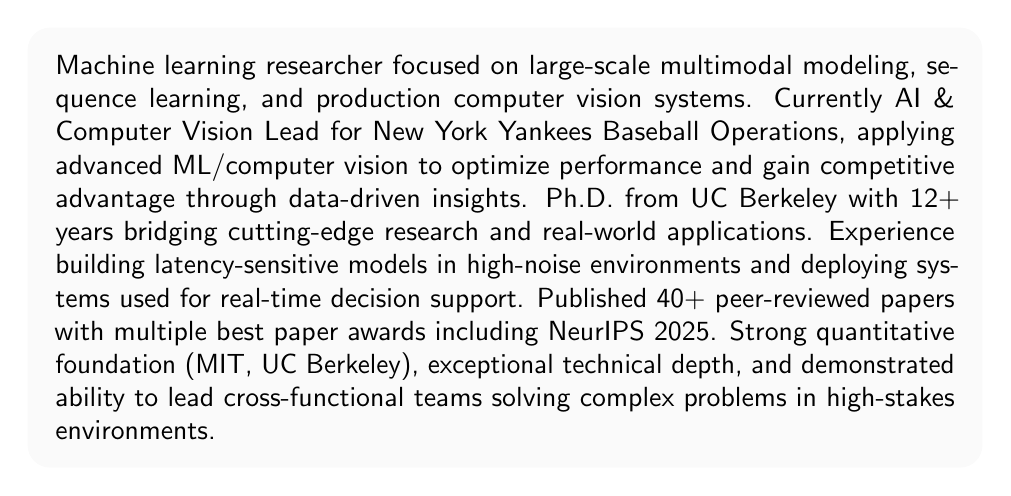
\begin{tikzpicture}
\node[fill=offWhite, rounded corners=8pt, inner sep=10pt, text width=\textwidth-20pt, align=justify] {
Machine learning researcher focused on large-scale multimodal modeling, sequence learning, and production computer vision systems. Currently AI \& Computer Vision Lead for New York Yankees Baseball Operations, applying advanced ML/computer vision to optimize performance and gain competitive advantage through data-driven insights. Ph.D. from UC Berkeley with 12+ years bridging cutting-edge research and real-world applications. Experience building latency-sensitive models in high-noise environments and deploying systems used for real-time decision support. Published 40+ peer-reviewed papers with multiple best paper awards including NeurIPS 2025. Strong quantitative foundation (MIT, UC Berkeley), exceptional technical depth, and demonstrated ability to lead cross-functional teams solving complex problems in high-stakes environments.
};
\end{tikzpicture}
\end{center}

\section{Education}
\begin{tabularx}{\textwidth}{@{}X r@{}}
\textbf{\color{darkGray}Ph.D., Computer Science} & \textcolor{mediumGray}{\textit{2013}} \\
\textcolor{mediumGray}{University of California, Berkeley} & \\[4pt]
\textbf{\color{darkGray}M.S., Computer Science} & \textcolor{mediumGray}{\textit{2010}} \\
\textcolor{mediumGray}{University of California, Berkeley} & \\[4pt]
\textbf{\color{darkGray}B.S., Computer Science} & \textcolor{mediumGray}{\textit{2003}} \\
\textcolor{mediumGray}{Massachusetts Institute of Technology} & \\
\end{tabularx}

\section{Professional Experience}

\profentry{AI \& Computer Vision Lead, Baseball Operations}{Dec. 2019 -- Present}{New York Yankees}{}
\begin{itemize}
\listentry{Lead applied ML/AI strategy for player performance optimization, injury prevention, and competitive intelligence in high-pressure, high-stakes environment requiring rapid iteration and measurable ROI}
\listentry{Deploy low-latency computer vision and sequence models for automated tracking and biomechanical inference across millions of video frames}
\listentry{Build forecasting models for high-variance, adversarial real-world environments; iterate rapidly on model improvements with direct performance impact}
\listentry{Optimize noisy multimodal data pipelines (video, sensors, biomechanics) for stability, robustness, and rapid retraining}
\listentry{Lead cross-functional teams of engineers, analysts, and domain experts in fast-paced, results-driven environment}
\end{itemize}

\vspace{4pt}
\profentry{Associate Professor (with Tenure)}{Sept. 2018 -- Present}{Rutgers University, Electrical and Computer Engineering}{}
\begin{itemize}
\listentry{Lead research group focused on multimodal deep learning, time-series modeling, and large-scale ML infrastructure}
\listentry{Develop sequence models, multimodal fusion architectures, and causal inference tools for large-scale real-world datasets}
\listentry{Published 40+ peer-reviewed papers in top-tier ML venues (NeurIPS, ICML workshops, ACM conferences) with multiple best paper awards for rigorous technical contributions}
\listentry{Mentor Ph.D. students on production ML systems: 3 graduates (2022-2023) now in industry research roles at major tech companies}
\end{itemize}

\vspace{4pt}
\profentry{Research Staff Member}{Dec. 2013 -- Aug. 2018}{IBM Research}{}
\begin{itemize}
\listentry{Advanced ML/AI systems for enterprise applications focusing on IoT analytics, predictive modeling, and large-scale data processing}
\listentry{Developed algorithms for forecasting and model robustness under nonstationary input regimes}
\listentry{Designed forecasting and anomaly detection models for complex time-series with distribution shift}
\listentry{12+ issued U.S. patents in machine learning, IoT sensing, and intelligent systems}
\end{itemize}

\vspace{4pt}
\profentry{Senior Software Engineer}{Jan. 2013 -- Sept. 2013}{Spire Global (Nanosatisfi)}{}
\begin{itemize}
\listentry{Early-stage startup: built core satellite communication software and data processing pipelines for nanosatellite constellation}
\end{itemize}

\vspace{4pt}
\profentry{Software Engineer}{Aug. 2003 -- Feb. 2007}{Oracle Corporation}{}
\begin{itemize}
\listentry{Developed enterprise database software and optimization algorithms for Oracle Database 10g/11g}
\end{itemize}

\section{Technical Expertise}

\begin{center}
\begin{tikzpicture}
\node[fill=offWhite, rounded corners=8pt, inner sep=10pt, text width=\textwidth-20pt, align=center] {
\textbf{\color{citadelBlue}Machine Learning} \textbullet\ 
\textbf{\color{citadelBlue}Computer Vision \& 3D Reconstruction} \textbullet\ 
\textbf{\color{citadelBlue}Deep Learning (CNNs, Transformers, GANs)}\\[2pt]
\textbf{\color{citadelBlue}Time-Series Analysis \& Forecasting} \textbullet\ 
\textbf{\color{citadelBlue}Statistical Modeling \& Optimization} \textbullet\ 
\textbf{\color{citadelBlue}Multimodal Learning}\\[2pt]
\textbf{\color{citadelBlue}Representation Learning} \textbullet\ 
\textbf{\color{citadelBlue}Sequence Modeling} \textbullet\ 
\textbf{\color{citadelBlue}Model Debugging \& Failure Mode Analysis}\\[2pt]
\textbf{\color{citadelBlue}Large-Scale Data Processing} \textbullet\ 
\textbf{\color{citadelBlue}Production ML Systems} \textbullet\ 
\textbf{\color{citadelBlue}Python, C/C++, PyTorch, TensorFlow}
};
\end{tikzpicture}
\end{center}

\section{Key Achievements \& Impact}

\begin{itemize}
\listentry{\textbf{\color{citadelBlue}Production ML Deployment}: Deployed production CV and sequence models used daily for high-stakes, real-time decision workflows}

\listentry{\textbf{\color{citadelBlue}NeurIPS 2025}: Developed autoregressive 3D occupancy model combining Gaussian splatting with sequential masking}

\listentry{\textbf{\color{citadelBlue}Best Paper Awards}: ICISSP 2018 (Award), IoTDI 2019 (Finalist), BuildSys 2015 (2× Finalist) -- Recognition for technically rigorous, high-impact research}

\listentry{\textbf{\color{citadelBlue}Innovation}: 12+ issued U.S. patents demonstrating technology transfer from research to production systems}
\end{itemize}

\section{Selected Publications (Machine Learning \& CV)}

\begin{itemize}[topsep=0pt]
\listentry{Y. Sun, J. Contreras, \textbf{J. Ortiz}, ``DFGauss: Dynamic Focused Masking for Autoregressive 3D Occupancy Prediction,'' \textit{NeurIPS}, 2025.}

\listentry{Y. Sun, N. Salami Pargoo, P. Jin, \textbf{J. Ortiz}, ``Optimizing Autonomous Driving for Safety: A Human-Centric Approach with LLM-Enhanced RLHF,'' \textit{ACM UbiComp Companion}, 2024.}

\listentry{\textbf{J. Ortiz}, C. Crawford, F. Le, ``DeviceMien: Network Device Behavior Modeling for Identifying Unknown IoT Devices,'' \textit{ACM IoTDI}, 2019. \textbf{\color{accentBlue}[Best Paper Finalist]}}

\listentry{T. Wu, N. Martelaro, S. Stent, \textbf{J. Ortiz}, W. Ju, ``Learning When Agents Can Talk to Drivers Using the INAGT Dataset and Multisensor Fusion,'' \textit{ACM IMWUT}, 2021.}
\end{itemize}

\section{Mentoring}
Mentor Ph.D. researchers working on multimodal ML and production systems: 3 graduates (2022-2023) now in industry research roles.

\vspace{6pt}
\begin{center}
\begin{tikzpicture}
\node[fill=citadelBlue!8, rounded corners=8pt, inner sep=8pt, text width=\textwidth-20pt, align=center] {
\textbf{\color{citadelBlue}Strengths:} Building robust ML systems from noisy real-world data \textbullet\ Fast iteration under uncertainty \textbullet\ Deploying deep learning models at scale
};
\end{tikzpicture}
\end{center}

\end{document}

